\documentclass[english, compress, red]{beamer}


\usetheme{Warsaw}
\usecolortheme{lily}
\useoutertheme[subsection=false]{smoothbars}
\useinnertheme{rectangles}

\setbeamertemplate{headline}{}

\usepackage{amsmath}
\usepackage{amsfonts}
\usepackage{amsthm}

%text encoding
\usepackage[english]{babel}

\usepackage{dcolumn}
\usepackage{booktabs}
\usepackage{tikz}
\usetikzlibrary{positioning,shapes,arrows}

\newcolumntype{M}[1]{D{.}{.}{1.#1}}

\usepackage{subcaption}

\usepackage{algorithm}
\usepackage{algpseudocode}


\usepackage[sort, round]{natbib}
\bibliographystyle{plainnat}

%\usepackage[style=authoryear, backend=biber]{biblatex}
%\addbibresource{references.bib}

\title{An Introduction to Maximal Ancestral Graphs}
\author{Nikolaos Kougioulis}
\institute{University of Crete \\Department of Computer Science \\ \vspace{6pt} CS-583}

\day=07\relax
\month=11\relax
\year=2023\relax

\newcommand{\indep}{\rotatebox[origin=c]{90}{$\models$}}
\DeclareMathOperator*{\argmax}{arg\,max}
\DeclareMathOperator*{\parent}{Par}

\begin{document}
	
	\frame{\titlepage}

\frame{\frametitle{Bayesian Networks} 
	\begin{definition}A \textbf{Bayesian Network (BN)} is a pair $(G,\Theta)$ where $G$ is a DAG between random variables $\mathcal{U} = \left\{X_1, \ldots, X_n \right\}$ and $\Theta$ a set of conditional probabilities $\theta_i = P(X_i | \text{Par}(X_i)) ~\forall X_i$. The joint probability on $\mathcal{U}$ decomposes according to the chain rules as 
		
	$$P(X_1,\ldots,X_n) = \prod_{i=1}^{n} P(X_i|\text{Par}{X_i})$$
	\end{definition}
}

\frame{\frametitle{Directed edges}
	\begin{itemize}
		\item A directed edge denotes dependence, whereas the absence of an edge denotes (conditional) independence.
		\item In the causal context, a directed edge $X \rightarrow Y$ denotes that $X$ is a \textbf{direct} cause of Y ($Y$ is a \textbf{direct} effect of $X$).
	\end{itemize}
}

\begin{frame}{Example (J. Pearl, 2009)}
		\begin{tikzpicture}[
			node distance=1cm and 0cm,
			mynode/.style={draw,ellipse,text width=2cm,align=center}
			]
			\node[mynode] (sp) {Sprinkler};
			\node[mynode,below right=of sp] (gw) {Grass wet};
			\node[mynode,above right=of gw] (ra) {Rain};
			\path (ra) edge[-latex] (sp)
			(sp) edge[-latex] (gw) 
			(gw) edge[latex-] (ra);
			\node[left=0.5cm of sp]
			{
				\begin{tabular}{cM{2}M{2}}
					\toprule
					& \multicolumn{2}{c}{Sprinkler} \\
					Rain & \multicolumn{1}{c}{T} & \multicolumn{1}{c}{F} \\
					\cmidrule(r){1-1}\cmidrule(l){2-3}
					F & 0.4 & 0.6 \\
					T & 0.01 & 0.99 \\
					\bottomrule
				\end{tabular}
			};
			\node[right=0.5cm of ra]
			{
				\begin{tabular}{M{1}M{1}}
					\toprule
					\multicolumn{2}{c}{Sprinkler} \\
					\multicolumn{1}{c}{T} & \multicolumn{1}{c}{F} \\
					\cmidrule{1-2}
					0.2 & 0.8 \\
					\bottomrule
				\end{tabular}
			};
			\node[below=0.5cm of gw]
			{
				\begin{tabular}{ccM{2}M{2}}
					\toprule
					& & \multicolumn{2}{c}{Grass wet} \\
					\multicolumn{2}{l}{Sprinkler rain} & \multicolumn{1}{c}{T} & \multicolumn{1}{c}{F} \\
					\cmidrule(r){1-2}\cmidrule(l){3-4}
					F & F & 0.4 & 0.6 \\
					F & T & 0.01 & 0.99 \\
					T & F & 0.01 & 0.99 \\
					T & T & 0.01 & 0.99 \\
					\bottomrule
				\end{tabular}
			};
		\end{tikzpicture}
\end{frame}

\begin{frame}{Markov Condition}	
	Denote conditional dependence (independence) of two non-empty sets of variables $\mathbf{X,Y} \subset \mathcal{V}$ given $\mathbf{Z} \subset \mathcal{V}\left\{ \mathbf{X,Y} \right\}$ (possibly empty)  as $Dep(\mathbf{X;Y | Z})$ ($Ind(\mathbf{X;Y | Z})$).
	
	\begin{definition}
		A node is conditionally independent of its nondescendants on the graph, given its parents.
	\end{definition}

    \begin{definition}
    	A node is conditionally independent of its non-effects on the graph, given its direct causes.
    \end{definition}

\end{frame}

\begin{frame}{Markov Condition - Example}
	\begin{columns}
		\begin{column}{0.6\textwidth}
			\begin{figure}
			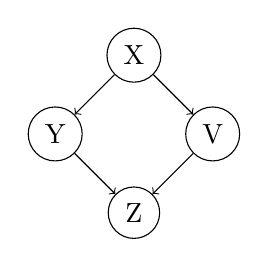
\begin{tikzpicture}
		\node[draw, circle] (X) at (0,0) {X};
		\node[draw, circle] (Y) at (-1,-1) {Y};
		\node[draw, circle] (Z) at (0,-2) {Z};
		\node[draw, circle] (V) at (1,-1) {V};
				
		\draw[->] (X) -- (Y);
		\draw[->] (Y) -- (Z);
		\draw[->] (V) -- (Z);
		\draw[->] (X) -- (V);

	\end{tikzpicture}
   \caption{Figure 1}
   \end{figure}
   \end{column}
   \begin{column}{0.4\textwidth}	
    \begin{itemize}
    	\item $Ind(Y;V|X)$
    	\item $Ind(Z;X | \left\{Y,V \right\})$
    	\item $Ind(X;Z | \emptyset)$
    	\item etc.
    \end{itemize}
    \end{column}
    \end{columns}
\end{frame}

\begin{frame}{Colliders and non-colliders}
	\begin{definition}A node $X$ of a path $p$ in the DAG is called a \textbf{collider} if the previous and next nodes of $X$ in the path are into $X$.
	\end{definition}

    \begin{definition}
    	A node $X$ of a path $p$ in the DAG is called an \textbf{unshielded collider} if the previous and next nodes $Y,Z$ of $X$ in the path are into $X$ and $Y$ and $Z$ are not adjacent.
    \end{definition}
\end{frame}

\begin{frame}{Colliders and non-colliders}
	\begin{definition}
		A path p from X to Y is \textbf{blocked} by a set of nodes $\mathbf{Z}$ (possibly empty), if some node on $p$:
		\begin{itemize}
		\item is a collider and neither it or any of its descendants are in $\mathbf{Z}$, or
		\item is not a collider and is in $\mathbf{Z}$
		\end{itemize}
	\end{definition}
    \begin{definition}
	If a path $p$ is not blocked by a set of nodes $\mathbf{Z}$, it is said to be \textbf{active}.
	\end{definition}

E.g The path $X-Y-Z$ is blocked by $\mathbf{Y}$, $Y-Z-V$ is blocked by $\mathbf{Z}=\emptyset$ etc.
\end{frame}

\begin{frame}{d-separation criterion}
	\begin{definition}Two nodes $X$ and $Y$ are d-separated by $\mathbf{Z}$ if-f every path from $X$ to $Y$ is blocked by $\mathbf{Z}$. Otherwise, we say they are \textbf{d-connected}.
	\end{definition}	
\end{frame}

\begin{frame}{Causal Faithfulness Assumption}
	Given a causally sufficient set of variables $\mathcal{U}$ in a population $N$, every conditional independence relation that holds in the density over $\mathcal{U}$ is entailed by the local directed Markov condition for the causal DAG of $N$.
\end{frame}

\begin{frame}{Causal Sufficiency}
	Assumption that there are unobserved variables.
	
	Unobserved variables are called \textbf{latent} or \textbf{hidden} variables.
	
\end{frame}

\begin{frame}[t]
	\frametitle{Graphs: X $\leftrightarrow$ L $\leftrightarrow$ Y and X $\leftrightarrow$ Y}
	\begin{columns}[onlytextwidth]
		\column{0.5\textwidth}
		\begin{center}
			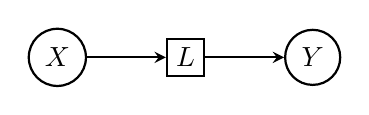
\begin{tikzpicture}[->,>=stealth,thick]
				% X -> L -> Y
				\node[draw, circle] (XLY1) {$X$};
				\node[draw, rectangle,right=of XLY1] (L1) {$L$};
				\node[draw, circle,right=of L1] (Y1) {$Y$};
				
				\draw[->] (XLY1) -- (L1);
				\draw[->] (L1) -- (Y1);
			\end{tikzpicture}
		\end{center}
		
		\column{0.5\textwidth}
		\begin{center}
			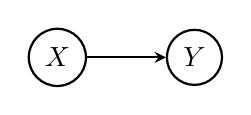
\begin{tikzpicture}[->,>=stealth,thick]
				% X <-> Y
				\node[draw, circle] (XY1) {$X$};
				\node[draw, circle,right=of XY1] (Y1) {$Y$};
				
				\draw[->] (XY1) -- (Y1);
			\end{tikzpicture}
		\end{center}
	\end{columns}
	
	\vspace{1em}
	
	\frametitle{Latent Confounders}
	\begin{columns}[onlytextwidth]
		\column{0.5\textwidth}
		\begin{center}
			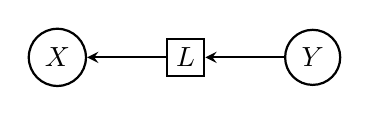
\begin{tikzpicture}[->,>=stealth,thick]
				% X <-> L <-> Y
				\node[draw, circle] (XLY2) {$X$};
				\node[draw, rectangle,right=of XLY2] (L2) {$L$};
				\node[draw, circle,right=of L2] (Y2) {$Y$};
				
				\draw[<-] (XLY2) -- (L2);
				\draw[<-] (L2) -- (Y2);
			\end{tikzpicture}
		\end{center}
		
		\column{0.5\textwidth}
		\begin{center}
			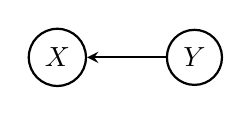
\begin{tikzpicture}[->,>=stealth,thick]
				% X <-> Y
				\node[draw, circle] (XY2) {$X$};
				\node[draw, circle,right=of XY2] (Y3) {$Y$};
				
				\draw[<-] (XY2) -- (Y3);
			\end{tikzpicture}
		\end{center}
	\end{columns}

    \begin{columns}[onlytextwidth]
    	\column{0.5\textwidth}
    	\begin{center}
    		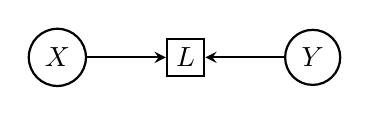
\begin{tikzpicture}[->,>=stealth,thick]
    			% X <-> L <-> Y
    			\node[draw, circle] (XLY2) {$X$};
    			\node[draw, rectangle,right=of XLY2] (L2) {$L$};
    			\node[draw, circle,right=of L2] (Y2) {$Y$};
    			
    			\draw[->] (XLY2) -- (L2);
    			\draw[<-] (L2) -- (Y2);
    		\end{tikzpicture}
    	\end{center}
    	
    	\column{0.5\textwidth}
    	\begin{center}
    		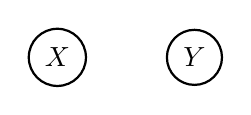
\begin{tikzpicture}[->,>=stealth,thick]
    			% X <-> Y
    			\node[draw, circle] (XY2) {$X$};
    			\node[draw, circle,right=of XY2] (Y3) {$Y$};
    
    		\end{tikzpicture}
    	\end{center}
    \end{columns}

     \begin{columns}[onlytextwidth]
    	\column{0.5\textwidth}
    	\begin{center}
    		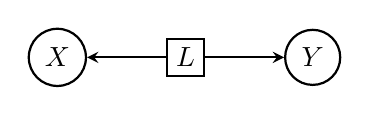
\begin{tikzpicture}[->,>=stealth,thick]
    			% X <-> L <-> Y
    			\node[draw, circle] (XLY2) {$X$};
    			\node[draw, rectangle,right=of XLY2] (L2) {$L$};
    			\node[draw, circle,right=of L2] (Y2) {$Y$};
    			
    			\draw[<-] (XLY2) -- (L2);
    			\draw[->] (L2) -- (Y2);
    		\end{tikzpicture}
    	\end{center}
    	
    	\column{0.5\textwidth}
    	\begin{center}
    		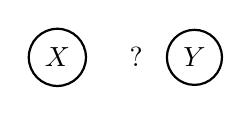
\begin{tikzpicture}[->,>=stealth,thick]
    			\node[draw, circle] (XY2) {$X$};
    			\node[draw, circle,right=of XY2] (Y3) {$Y$};
    			\node at (1,0) {?};
    		\end{tikzpicture}
    	\end{center}
    \end{columns}
	
\end{frame}


\begin{frame}{Latent Confounders}
	
	
	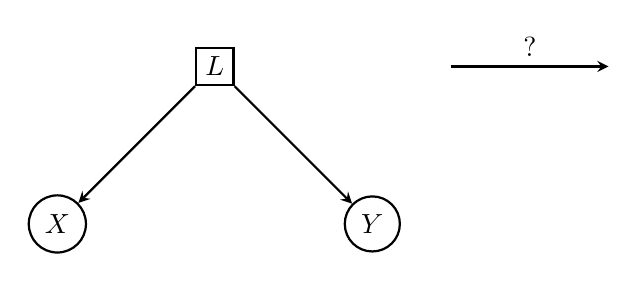
\begin{tikzpicture}[->,>=stealth,thick]
		\node[draw, rectangle] (L) at (0, 1) {$L$};
		\node[draw, circle] (X) at (-2, -1) {$X$};
		\node[draw, circle] (Y) at (2, -1) {$Y$};
		
		\path (L) edge (X);
		\path (L) edge (Y);
		
		\draw[->] (3, 1) -- (5, 1) node[midway, above] {?};
		
	\end{tikzpicture}

    \vspace{29pt}
	
	$X$ and $Y$ are not independent.
	No edge $X$ and $Y$ represents their independence relation correctly.
	
\end{frame}

\begin{frame}{Mixed Graphs}
	\begin{definition}A (directed) \textbf{mixed graph} $\mathcal{G}$ is a graph that may contain two kinds of edges: directed edges ($\rightarrow$) and bi-directed edges ($\leftrightarrow$).
	\end{definition}

    \begin{itemize}
    	\item Between any two vertices there is at \textbf{most one edge}.
    	\item The two ends of an edge we call \textbf{marks}.
    	\item There are two kinds of marks: \textbf{arrowhead} ($>$) and \textbf{tail} ($-$).
    	\item We say an edge is \textbf{into} (\textbf{out of}) a vertex if the mark of the edge at the vertex is an arrowhead (or tail).
    \end{itemize}
\end{frame}

\begin{frame}{Mixed Graphs}
	If
	\begin{equation*}
			\begin{cases}
				X \leftrightarrow Y \\
				X \rightarrow Y \\
				X \leftarrow Y
			\end{cases}
			\text{in} ~\mathcal{M} ~\text{then} ~X ~\text{is a}
			\begin{cases}
				\textbf{spouse} \\
				\textbf{parent} \\
				\textbf{child}
			\end{cases}
			\text{of} ~Y ~\text{and}
			\begin{cases}
				X \in \textbf{sp}(Y) \\
				X \in \textbf{pa}(Y) \\
				X \in \textbf{ch}(Y)
			\end{cases}
	\end{equation*}
	
	\begin{definition}
		A vertex $X$ is said to be an \textbf{ancestor} of a vertex $Y$, denoted $X \in \textbf{an}(Y)$, if either there exists a directed path $X \rightarrow \cdots \rightarrow Y$ from $X$ to $Y$, or $X=Y$.
	\end{definition}
\end{frame}

\begin{frame}{Ancestral Graphs}
	\begin{definition}A mixed (directed) graph is an \textbf{ancestral graph} if:
		\begin{itemize}
			\item there are no directed cycles;
			\item whenever there is an edge $X \leftrightarrow Y$, then there is no directed path from $X$ to $Y$ or from $Y$ to $X$ (no almost directed cycles)
		\end{itemize}
	\end{definition}

\begin{figure}
\begin{subfigure}{0.48\textwidth}
	\centering
	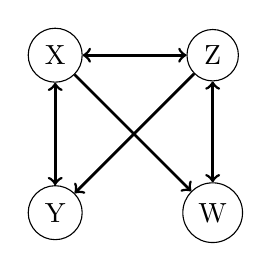
\begin{tikzpicture}
		\node[circle, draw] (X1) at (0, 0) {X};
		\node[circle, draw] (Z1) at (2, 0) {Z};
		\node[circle, draw] (Y1) at (0, -2) {Y};
		\node[circle, draw] (W1) at (2, -2) {W};
		\draw[->, line width=1pt] (X1) -- (W1);
		\draw[<->, line width=1pt] (Z1) -- (W1);
		\draw[->, line width=1pt] (Z1) -- (Y1);
		\draw[<->, line width=1pt] (X1) -- (Y1);
		\draw[<->, line width=1pt] (Z1) -- (X1); 
	\end{tikzpicture}
	\caption{An ancestral graph.}
\end{subfigure}
\hfill
\begin{subfigure}{0.48\textwidth}
	\centering
	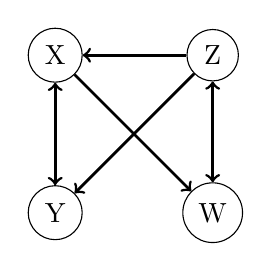
\begin{tikzpicture}
		\node[circle, draw] (X2) at (0, 0) {X};
		\node[circle, draw] (Z2) at (2, 0) {Z};
		\node[circle, draw] (Y2) at (0, -2) {Y};
		\node[circle, draw] (W2) at (2, -2) {W};
		\draw[->, line width=1pt] (X2) -- (W2);
		\draw[<->, line width=1pt] (Z2) -- (W2);
		\draw[->, line width=1pt] (Z2) -- (Y2);
		\draw[<->, line width=1pt] (X2) -- (Y2);
		\draw[->, line width=1pt] (Z2) -- (X2);
	\end{tikzpicture}
	\caption{Not an ancestral graph.}
\end{subfigure}
\end{figure}
\end{frame}

\begin{frame}{Collider Paths in AGs}
	\begin{definition}
		\begin{itemize}
			\item In an ancestral graph, a nonendpoint vertex X on a path is said to be a \textbf{collider} if two arrowheads meet at X (i.e., $\rightarrow X \leftarrow, \leftrightarrow X \leftrightarrow, \leftrightarrow X \leftarrow. \rightarrow X \leftrightarrow$).
		    \item All other nonendpoint vertices on a path are called \textbf{noncolliders} (i.e., $\rightarrow X \rightarrow, \leftarrow X \leftarrow, \leftarrow X \rightarrow, \leftrightarrow X \rightarrow, \leftarrow X \leftrightarrow$)
			\item A path along which every nonendpoint is a collider is called a \textbf{collider path}.
		\end{itemize}
	\end{definition}
\end{frame}

\begin{frame}{m-Connecting Paths}
	\begin{definition}In an ancestral graph, a path $\pi$ between vertices $X$ and $Y$ is active or $\textbf{m-connecting}$ relative to a (possibly empty) set of vertices $\textbf{Z}$, with $X,Y \not \in \mathbf{Z}$ if 
		
		\begin{itemize}
			\item every non-collider on $\pi$ is not a member of $\mathbf{Z}$
			\item every collider on $\pi$ is an ancestor of some member of $\mathbf{Z}$
		\end{itemize}
	Otherwise we say that $\mathbf{Z}$ \textbf{blocks} $\pi$.
	\end{definition}\

Example: For the ancestral graph $A \rightarrow B \leftrightarrow C \leftarrow D$:
\begin{itemize}
	\item The path $\pi_1 = (A,B,C,D)$ is active relative to $\mathbf{Z} = \left\{ B,C \right\}$
	\item The path $\pi_1$ is not m-connecting relative to $\mathbf{Z} = \emptyset$, $\mathbf{Z} = \left\{ B \right\}$ or $\mathbf{Z} = \left\{ C\right\}$.
\end{itemize}
\end{frame}

\begin{frame}{m-Separation}
	\begin{definition}
		\begin{itemize}
			\item $X$ and $Y$ are said to be \textbf{m-separated by} $\mathbf{Z}$ if there are no active paths between $X$ and $Y$ relative to $\mathbf{Z}$, i.e if $\mathbf{Z}$ blocks all paths between $X$ and $Y$.
			\item Two disjoint sets of variables $X$ and $Y$ are m-separated by $\mathbf{Z}$ if every variable in $\mathbf{X}$ is m-separated from every variable in $\mathbf{Y}$ by $\mathbf{Z}$.
		\end{itemize}
	\end{definition}
Example: For the ancestral graph $A \rightarrow B \leftarrow C \leftarrow D$:
\begin{itemize}
	\item $\left\{ A\right\} \perp\!\!\!\perp_m \left\{ D \right\}$ \\
	$\left\{ A\right\} \perp\!\!\!\perp_m \left\{ D \right\} | \left\{ B \right\}$ \\
	$\left\{ A\right\} \perp\!\!\!\perp_m \left\{ D \right\} | \left\{ C\right\}$ 
	
	since there is no active path relative to $\mathbf{Z} = \emptyset$, $\mathbf{Z} = \left\{ B \right\}$ and $\mathbf{Z} = \left\{ C \right\}$ respectively.
	
	\item $\left\{ A\right\} \not \perp\!\!\!\perp_m \left\{ D \right\} | \left\{ B, C\right\}$ because $\pi_1 = (A,B,C,D)$ is active relative to $\mathbf{Z} = \left\{ B,C \right\}$
\end{itemize}
\end{frame}

\begin{frame}{Pairwise Markov property}
	Every missing edge corresponds to a conditional independence relation. 

	\begin{definition}
		An ancestral graph is \textbf{maximal} if for every pair of nonadjacent vertices $(a, b)$ there exists a set $\mathbf{Z}$ with $a, b \not \in \mathbf{Z}$ such that $a$ and $b$ are m-separated conditional on $\mathbf{Z}$ (i.e the pairwise Markov property holds).
	\end{definition}
	
\end{frame}

\begin{frame}{Maximal Ancestral Graphs}
	\begin{definition}
		An ancestral graph $\mathcal{G}$ is said to be \textbf{maximal} if for every pair of non-adjacent vertices $(X,Y)$ there exists a set of $\mathbf{Z}$ ($X,Y \not \in \mathbf{Z}$) such that $X$ and $Y$ are m-separated conditional on $\mathbf{Z}$.
	\end{definition}
    \begin{figure}
    	\begin{subfigure}{0.48\textwidth}
    		\centering
    		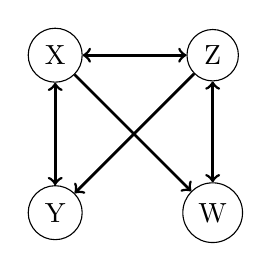
\begin{tikzpicture}
    			\node[circle, draw] (X1) at (0, 0) {X};
    			\node[circle, draw] (Z1) at (2, 0) {Z};
    			\node[circle, draw] (Y1) at (0, -2) {Y};
    			\node[circle, draw] (W1) at (2, -2) {W};
    			\draw[->, line width=1pt] (X1) -- (W1);
    			\draw[<->, line width=1pt] (Z1) -- (W1);
    			\draw[->, line width=1pt] (Z1) -- (Y1);
    			\draw[<->, line width=1pt] (X1) -- (Y1);
    			\draw[<->, line width=1pt] (Z1) -- (X1);
    		\end{tikzpicture}
    		\caption{A not maximal ancestral graph.}
    	\end{subfigure}
    	\hfill
    	\begin{subfigure}{0.48\textwidth}
    		\centering
    		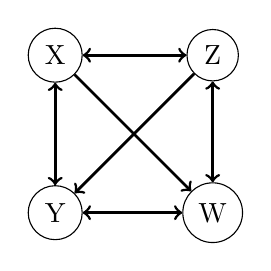
\begin{tikzpicture}
    			\node[circle, draw] (X1) at (0, 0) {X};
    			\node[circle, draw] (Z1) at (2, 0) {Z};
    			\node[circle, draw] (Y1) at (0, -2) {Y};
    			\node[circle, draw] (W1) at (2, -2) {W};
    			\draw[->, line width=1pt] (X1) -- (W1);
    			\draw[<->, line width=1pt] (Z1) -- (W1);
    			\draw[->, line width=1pt] (Z1) -- (Y1);
    			\draw[<->, line width=1pt] (X1) -- (Y1);
    			\draw[<->, line width=1pt] (Z1) -- (X1);
    			\draw[<->, line width=1pt] (Y1) -- (W1);
    		\end{tikzpicture}
    		\caption{A maximal ancestral graph.}
    	\end{subfigure}
    \end{figure}
\end{frame}

\begin{frame}{Maximal Ancestral Graphs}
	\begin{columns}
		\begin{column}{0.3\textwidth}
			\centering
			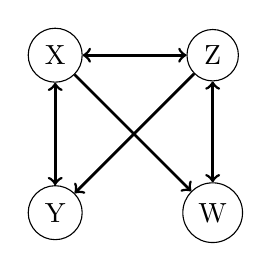
\begin{tikzpicture}
				\node[circle, draw] (X1) at (0, 0) {X};
				\node[circle, draw] (Z1) at (2, 0) {Z};
				\node[circle, draw] (Y1) at (0, -2) {Y};
				\node[circle, draw] (W1) at (2, -2) {W};
				\draw[->, line width=1pt] (X1) -- (W1);
				\draw[<->, line width=1pt] (Z1) -- (W1);
				\draw[->, line width=1pt] (Z1) -- (Y1);
				\draw[<->, line width=1pt] (X1) -- (Y1);
				\draw[<->, line width=1pt] (Z1) -- (X1); 
			\end{tikzpicture}
		\end{column}
	     \begin{column}{0.7\textwidth}
	     	To show that the AG is indeed maximal, notice that the only pair of non-adjacent vertices is $(Y,W)$.
	     	\begin{itemize}
	     		\item $\mathbf{Z} = \left\{ X\right\}$, $\pi_1$ is \textit{not an active path} since $Z \not \in \textbf{an}(X)$ but $\pi_2 = (Y,Z,W)$ is active since there are no colliders in $\pi_2$, $Z$ is a non-collider for $\pi_2$ and $Z \not \in \mathbf{Z}$
	     		\item For $\mathbf{Z} = \left\{ X, Z\right\}$, $\pi_1 = (Y,X,Z,W)$ is a path that m-connects $Y$ and $W$.
	     		\item For $\mathbf{Z} = \left\{ Z\right\}$, $\pi_3 = (Y,Z,W)$ is an active path as there are no colliders in $\pi_3$, $X$ is a non-collider for $\pi_3$ and $X \not \in \mathbf{Z}$.
	     		\item For $\mathbf{Z} = \emptyset$, $\pi_1$ and $\pi_3$ are active paths.
	     	\end{itemize}
	     \end{column}
	\end{columns}
\end{frame}

\begin{frame}{Meaning of edges in a MAG}
	\begin{theorem}
		A directed edge $X \rightarrow Y$ from some node $X$ into another node $Y$ denotes that $Y$ is not an ancestor of $X$.
	\end{theorem}
	\begin{proof}
		Let $\mathcal{M}$ be a MAG and $X,Y$ two nodes on $\mathcal{M}$. Assume $X \rightarrow Y$ is in $\mathcal{M}$ and $Y$ is an ancestor of $X$. Then there is a directed path from $Y$ to $X$, but this means that the MAG $\mathcal{G}$ contains a directed cycle, contradiction. Hence if $X \rightarrow Y$, $Y$ is not an ancestor of $X$.
	\end{proof}
	Similarly if $X \leftarrow Y$, $X$ is not an ancestor of $Y$.
	
\end{frame}


\begin{frame}{Meaning of edges in a MAG}
	With a similar proof as before, we can show that 
	
	\begin{theorem}A bidirected edge $X \leftrightarrow Y$ between some nodes $X$ and $Y$ denotes that 
		\begin{itemize}
			\item $X$ is not an ancestor of $Y$
			\item $Y$ is not an ancestor of $X$
		\end{itemize}
	\end{theorem}
\end{frame}

\begin{frame}{Meaning of edges in a MAG}
	$X \rightarrow Y$:
	\begin{itemize}
		\item $X$ is an ancestor of $Y$
		\item $Y$ is \textit{not} an ancestor of $X$
		\item The above does not rule out \textbf{possible latent confounding} between $X$ and $Y$.
	\end{itemize}
	$X \leftrightarrow Y$:
	\begin{itemize}
		\item $X$ is \textit{not} an ancestor of $Y$
		\item $Y$ is \textit{not} an ancestor of $X$
		\item $X$ and $Y$ are \textbf{confounded}.
	\end{itemize}
\end{frame}

\begin{frame}{Maximal Ancestral Graphs}
	Maximal ancestral graphs (MAGs) are maximal in the sense that \textbf{no additional edge may be added to the graph without changing the independence model}.
	
	\begin{theorem}If $\mathcal{M} = (V,E)$ is a maximal ancestral graph and $\mathcal{M}$ is a subgraph of $\mathcal{G}^* = (V,E^*)$, then $\mathbf{I}_m (\mathcal{M}) = \mathbf{I}_m(\mathcal{M}^*)$ implies that $\mathcal{M} = \mathcal{M}^*$.
	\end{theorem}
\end{frame}

\begin{frame}{Maximal Ancestral Graphs}
	\begin{theorem}If $\mathcal{G}$ is an ancestral graph then there exists a \textbf{unique} maximal ancestral graph $\mathcal{M}$ formed by adding $\leftrightarrow$ edges to $\mathcal{G}$ such that $\mathbf{I}_m (\mathcal{M}) = \mathbf{I}_m(\mathcal{G})$
	\end{theorem}
	
	 \begin{figure}
		\begin{subfigure}{0.48\textwidth}
			\centering
			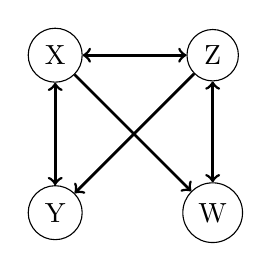
\begin{tikzpicture}

				\node[circle, draw] (X1) at (0, 0) {X};
				\node[circle, draw] (Z1) at (2, 0) {Z};
				\node[circle, draw] (Y1) at (0, -2) {Y};
				\node[circle, draw] (W1) at (2, -2) {W};
				\draw[->, line width=1pt] (X1) -- (W1);
				\draw[<->, line width=1pt] (Z1) -- (W1);
				\draw[->, line width=1pt] (Z1) -- (Y1);
				\draw[<->, line width=1pt] (X1) -- (Y1);
				\draw[<->, line width=1pt] (Z1) -- (X1);
			\end{tikzpicture}
			\caption{An ancestral graph $\mathcal{G}$.}
		\end{subfigure}
		\hfill
		\begin{subfigure}{0.48\textwidth}
			\centering
			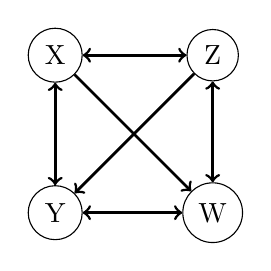
\begin{tikzpicture}
				\node[circle, draw] (X1) at (0, 0) {X};
				\node[circle, draw] (Z1) at (2, 0) {Z};
				\node[circle, draw] (Y1) at (0, -2) {Y};
				\node[circle, draw] (W1) at (2, -2) {W};
				\draw[->, line width=1pt] (X1) -- (W1);
				\draw[<->, line width=1pt] (Z1) -- (W1);
				\draw[->, line width=1pt] (Z1) -- (Y1);
				\draw[<->, line width=1pt] (X1) -- (Y1);
				\draw[<->, line width=1pt] (Z1) -- (X1);
				\draw[<->, line width=1pt] (Y1) -- (W1);
			\end{tikzpicture}
			\caption{The maximal ancestral graph $\mathcal{M}$ from $\mathcal{G}$.}
		\end{subfigure}
	\end{figure}
\end{frame}

\begin{frame}{Inducing Paths}
	Maximality is closely related to the definition of primitive inducing paths.
	
	\begin{definition}
		An \textbf{inducing path $\pi$ relative to a set} $\mathbf{L}$ between two vertices $X$ and $Y$ in an ancestral graph $\mathcal{G}$, is a path on which every non-endpoint vertex, \textit{not} in $\mathbf{L}$ is both a collider on $\pi$ and an ancestor of \textit{at least one} of the endpoints $X$ and $Y$.
	\end{definition}
    \begin{itemize}
    	\item Any single-edge path is trivially an inducing path relative to any set of vertices.
    	\item To simplify terminology, we will henceforth refer to inducing paths relative to the empty set simply as \textbf{inducing paths}.
    \end{itemize}
\end{frame}

\begin{frame}{Example}
	\begin{columns}
			\begin{column}{0.3\textwidth}
			\centering
			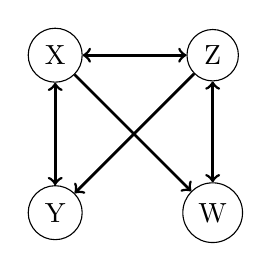
\begin{tikzpicture}
				\node[circle, draw] (X1) at (0, 0) {X};
				\node[circle, draw] (Z1) at (2, 0) {Z};
				\node[circle, draw] (Y1) at (0, -2) {Y};
				\node[circle, draw] (W1) at (2, -2) {W};
				\draw[->, line width=1pt] (X1) -- (W1);
				\draw[<->, line width=1pt] (Z1) -- (W1);
				\draw[->, line width=1pt] (Z1) -- (Y1);
				\draw[<->, line width=1pt] (X1) -- (Y1);
				\draw[<->, line width=1pt] (Z1) -- (X1);
			\end{tikzpicture}
		\end{column}
		\begin{column}{0.7\textwidth}
			\begin{itemize}
				\item The path $(Y,Z,W)$ is an inducing path relative to $\left\{ Z\right\}$ but not an inducing path relative to the empty set (because $Z$ is not a collider)
				\item The path $(Y,X,Z,W)$ is an inducing path relative to the empty set, because both $X$ and $Z$ are colliders on the path, $X$ is an ancestor of $W$ and $Z$ is an ancestor of $Y$.
			\end{itemize}
		\end{column}
	\end{columns}
\end{frame}

\begin{frame}{Alternative definition of MAGs}
	\begin{definition}A mixed graph is called a maximal ancestral graph (MAG) if:
		\begin{itemize}
			\item The graph does not contain any directed or almost directed cycles (ancestral) and
			\item there is \textit{no inducing path} between any two non-adjacent vertices (maximal)
		\end{itemize}
	\end{definition}
	\vspace{3pt}
	\begin{columns}
		\begin{column}{0.3\textwidth}
			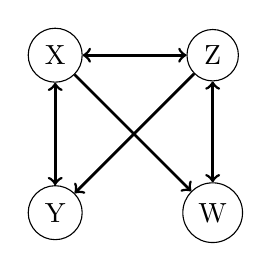
\begin{tikzpicture}
				\node[circle, draw] (X1) at (0, 0) {X};
				\node[circle, draw] (Z1) at (2, 0) {Z};
				\node[circle, draw] (Y1) at (0, -2) {Y};
				\node[circle, draw] (W1) at (2, -2) {W};
				\draw[->, line width=1pt] (X1) -- (W1);
				\draw[<->, line width=1pt] (Z1) -- (W1);
				\draw[->, line width=1pt] (Z1) -- (Y1);
				\draw[<->, line width=1pt] (X1) -- (Y1);
				\draw[<->, line width=1pt] (Z1) -- (X1);
			\end{tikzpicture}
		\end{column}
	\begin{column}{0.7\textwidth}
		The ancestral graph is not maximal because the path $(Y,X,Z,W)$ is an inducing path between the non-adjacent vertices $Y$ and $W$ ($X$ and $Z$ are colliders on the path and $X,Z$ ancestors of $Z$ and $Y$ respectively).
	\end{column}
	\end{columns}
\end{frame}

\begin{frame}{DAGs to MAGs}
	A property of MAGs is that they represent the marginal independence models of a DAG over $\mathbf{V} = \mathbf{O} \cup \mathbf{L}$. \\
		
	This means that given any DAG $\mathcal{D}$ over $\mathbf{V} = \mathbf{O}\cup \mathbf{L}$ there is a MAG $\mathcal{M}$ over $\mathbf{O}$ alone, such that for any disjoint sets $\mathbf{X, Y, Z \subset O, X}$ and $\mathbf{Y}$ are d-separated by $\mathbf{Z}$ in $\mathcal{D}$ if-f they are m-separated by $\mathbf{Z}$ in the MAG $\mathcal{M}$. \\
		
	This can be cosntructed with the following algorithm:
\end{frame}

\begin{frame}
	\frametitle{Constructing a MAG from a DAG}
	\begin{algorithm}[H]
		\caption{DAGs to MAGs}
		\begin{algorithmic}[1]
			\Require A DAG $\mathcal{D}$ over $\mathbf{O} \cup \mathbf{L}$
			\Ensure A MAG $\mathcal{M}_\mathcal{D}$ over $\mathbf{O}$
			\ForAll{pairs of variables $X, Y \in \mathbf{O}$}
			\State $\mathcal{M}$ is adjacent to $X$ and $Y$ if-f there is an inducing path between them relative to $\mathbf{L}$ in $\mathcal{D}$
			\EndFor
			\ForAll{pairs of adjacent variables $X, Y$ in $\mathcal{M}$}
			\If{$X$ is an ancestor of $Y$ in $\mathcal{D}$}
			\State Orient the edge as $X \to Y$ in $\mathcal{M}$
			\ElsIf{$Y$ is an ancestor of $X$ in $\mathcal{D}$}
			\State Orient the edge as $X \leftarrow Y$ in $\mathcal{M}$
			\Else
			\State Orient the edge as $X \leftrightarrow Y$ in $\mathcal{M}$
			\EndIf
			\EndFor
		\end{algorithmic}
	\end{algorithm}
\end{frame}

\begin{frame}{Example}
\begin{figure}
\begin{subfigure}{0.48\textwidth}
	\centering
	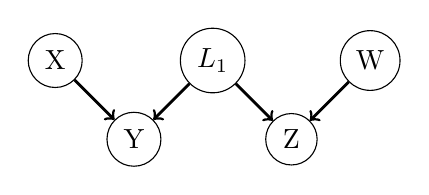
\begin{tikzpicture}
		\node[circle, draw] (X) at (0, 0) {X};
		\node[circle, draw] (Y) at (1, -1) {Y};
		\node[circle, draw] (L1) at (2, 0) {$L_1$};
		\node[circle, draw] (Z) at (3, -1) {Z};
		\node[circle, draw] (W) at (4, 0) {W};
		\draw[->, line width=1pt] (X) -- (Y);
		\draw[->, line width=1pt] (L1) -- (Y);
		\draw[->, line width=1pt] (L1) -- (Z);
		\draw[->, line width=1pt] (W) -- (Z);
	\end{tikzpicture}
	\caption{A DAG $\mathcal{D}$ over $\mathbf{O\cup L}$ where $\mathbf{L} = \left\{ L_1\right\}$.}
\end{subfigure}
\hfill
\begin{subfigure}{0.48\textwidth}
	\centering
	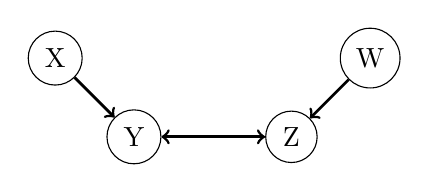
\begin{tikzpicture}
		\node[circle, draw] (X) at (0, 0) {X};
		\node[circle, draw] (Y) at (1, -1) {Y};
		\node[circle, draw] (Z) at (3, -1) {Z};
		\node[circle, draw] (W) at (4, 0) {W};
		\draw[->, line width=1pt] (X) -- (Y);
		\draw[<->, line width=1pt] (Y) -- (Z);
		\draw[->, line width=1pt] (W) -- (Z);
	\end{tikzpicture}
	\caption{A MAG $\mathcal{D}$ over $\mathbf{O}$ from the DAG $\mathcal{D}$.}
\end{subfigure}
\end{figure}
\end{frame}

\begin{frame}{Example}
	\begin{figure}
		\begin{subfigure}{0.48\textwidth}
			\centering
			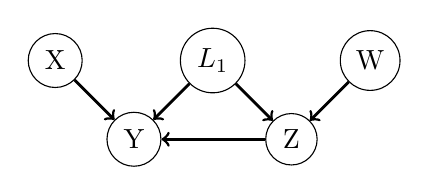
\begin{tikzpicture}
				\node[circle, draw] (X) at (0, 0) {X};
				\node[circle, draw] (Y) at (1, -1) {Y};
				\node[circle, draw] (L1) at (2, 0) {$L_1$};
				\node[circle, draw] (Z) at (3, -1) {Z};
				\node[circle, draw] (W) at (4, 0) {W};
				\draw[->, line width=1pt] (X) -- (Y);
				\draw[->, line width=1pt] (L1) -- (Y);
				\draw[->, line width=1pt] (L1) -- (Z);
				\draw[->, line width=1pt] (Z) -- (Y);
				\draw[->, line width=1pt] (W) -- (Z);
			\end{tikzpicture}
			\caption{A DAG $\mathcal{D}$ over $\mathbf{O\cup L}$ where $\mathbf{L} = \left\{ L_1\right\}$.}
		\end{subfigure}
		\hfill
		\begin{subfigure}{0.48\textwidth}
			\centering
			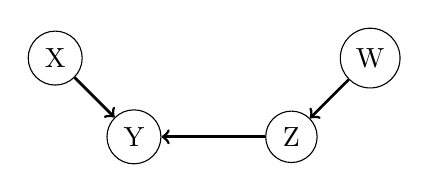
\begin{tikzpicture}
				\node[circle, draw] (X) at (0, 0) {X};
				\node[circle, draw] (Y) at (1, -1) {Y};
				\node[circle, draw] (Z) at (3, -1) {Z};
				\node[circle, draw] (W) at (4, 0) {W};
				\draw[->, line width=1pt] (X) -- (Y);
				\draw[->, line width=1pt] (Z) -- (Y);
				\draw[->, line width=1pt] (W) -- (Z);
			\end{tikzpicture}
			\caption{A MAG $\mathcal{D}$ over $\mathbf{O}$ from the DAG $\mathcal{D}$.}
		\end{subfigure}
	\end{figure}
\end{frame}

\begin{frame}{Example}
	\begin{figure}
		\begin{subfigure}{0.48\textwidth}
			\centering
			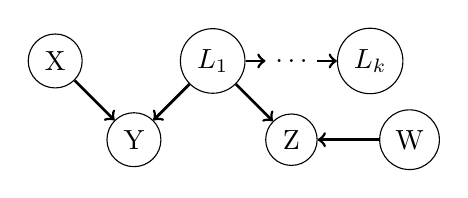
\begin{tikzpicture}
				\node[circle, draw] (X) at (0, 0) {X};
				\node[circle, draw] (Y) at (1, -1) {Y};
				\node[circle, draw] (L1) at (2, 0) {$L_1$};
				\node[] (dots) at (3,0) {$\ldots$};
				\node[circle, draw] (Lk) at (4,0) {$L_k$};
				\node[circle, draw] (Z) at (3, -1) {Z};
				\node[circle, draw] (W) at (4.5, -1) {W};
				\draw[->, line width=1pt] (X) -- (Y);
				\draw[->, line width=1pt] (L1) -- (Y);
				\draw[->, line width=1pt] (L1) -- (Z);
				\draw[->, line width=1pt] (W) -- (Z);
				\draw[->, line width=1pt] (L1) -- (dots);
				\draw[->, line width=1pt] (dots) -- (Lk);
			\end{tikzpicture}
			\caption{A DAG $\mathcal{D}$ over $\mathbf{O\cup L}$ where $\mathbf{L} = \left\{ L_1, \ldots, L_k \right\}$.}
		\end{subfigure}
		\hfill
		\begin{subfigure}{0.48\textwidth}
			\centering
			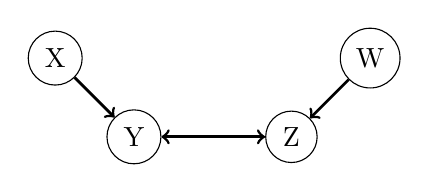
\begin{tikzpicture}
				\node[circle, draw] (X) at (0, 0) {X};
				\node[circle, draw] (Y) at (1, -1) {Y};
				\node[circle, draw] (Z) at (3, -1) {Z};
				\node[circle, draw] (W) at (4, 0) {W};
				\draw[->, line width=1pt] (X) -- (Y);
				\draw[<->, line width=1pt] (Y) -- (Z);
				\draw[->, line width=1pt] (W) -- (Z);
			\end{tikzpicture}
			\caption{A MAG $\mathcal{D}$ over $\mathbf{O}$ from the DAG $\mathcal{D}$.}
		\end{subfigure}
	\end{figure}
\end{frame}

\begin{frame}{Comments on edges on MAGs}
	\begin{itemize}
		\item Notice that as before, if two variables share a hidden common cause and there is a directed edge between them, then the MAG only keeps the directed edge.
		\item Because MAGs represent ancestral relationships, a directed edge dominates a bi-directed edge.
		\item There may also exist edges in the MAG that are not present in the underlying causal model
	\end{itemize}
\end{frame}

\begin{frame}{Markov Equivalence}
		Several MAGs can encode the same conditional independencies via m-separation (as various DAGs can encode the same conditional independencies via d-separation) and are not distinguishable only by correlational patterns.
		
		\begin{definition}Two MAGs $\mathcal{G}_1,\mathcal{G}\_2$ over the same set of vertices are called \textbf{Markov equivalent} if for any three
			disjoint sets of vertices $X,Y,Z$, $X$ and $Y$ are m-separated by $Z$ in $\mathcal{G}_1$ iff $X$ and $Y$ are m-separated by $Z$ in $\mathcal{G}_2$.
		\end{definition}
\end{frame}

\begin{frame}{Unshielded colliders}
	\begin{definition}In a MAG, a path consisting of a triple of vertices $X,Y,Z$ is said to be \textbf{unshielded} if $X$ and $Z$ are not adjacent.
	\end{definition}

    \begin{definition}A vertex $Y$ is called an \textbf{unshielded collider} if the vertices $X, Z$ are into $Y$ and $X$ and $Z$ are not adjacent.
    \end{definition}
\end{frame}

\begin{frame}{Discriminating paths}
	\begin{definition}In a MAG $\mathcal{G}$, a path $\pi = (x, q_1,\ldots, q_p,b, y), ~p \geq 1$ is called a \textbf{discriminating path for} $(q_p, b, y)$ if:
		\begin{itemize}
			\item $x$ is not adjacent to $y$, and
			\item every vertex $q_i$, $1 \leq i \leq p$ is a collider on $\pi$ and a parent of $y$.
		\end{itemize}
	\end{definition}
\end{frame}

\begin{frame}{Markov Equivalence in DAGs}
	It is known due to \cite{verma1990equivalence} that:
	\begin{theorem} Two DAGs $\mathcal{G}_1$ and $\mathcal{G}_2$ are Markov equivalent iff
		\begin{itemize}
			\item $\mathcal{G}_1$ and $\mathcal{G}_2$ have the same adjacencies
			\item $\mathcal{G}_1$ and $\mathcal{G}_2$ have the same unshielded colliders
		\end{itemize}
	\end{theorem}
\end{frame}
 
\begin{frame}{Markov Equivalence in MAGs}
	The following is known as the Spirtes and Richardson Criterion (SRC) (\cite{spirtes1996polynomial}):
	
	\begin{theorem}
		 Two MAGs $\mathcal{G}_1$ and $\mathcal{G}_2$ are Markov equivalent iff
		 \begin{itemize}
		 	\item $\mathcal{G}_1$ and $\mathcal{G}_2$ have the same adjacencies
		 	\item $\mathcal{G}_1$ and $\mathcal{G}_2$ have the same unshielded colliders and
		 	\item if $\pi$ forms a discriminating path for $b$ in $\mathcal{G}_1$ and $\mathcal{G}_2$, then $b$ is a collider on the path $\pi$ in $\mathcal{G}_1$ if and only if it is a collider on the path $\pi$ in $\mathcal{G}_2$.
		 \end{itemize}
	\end{theorem}
\end{frame}

\begin{frame}{Markov Equivalence}
	\begin{itemize}
	    \item Markov Equivalent MAGs form a Markov equivalence class that can be described uniquely by a \textbf{partial ancestral graph (PAG)}.
	    \item A PAG $\mathcal{P}$ has the same adjacencies as any MAG in the Markov equivalence class described by $\mathcal{P}$.
	    \item We denote all MAGs in the Markov equivalence class described by a PAG $\mathcal{G}$ by $[\mathcal{G}]$.
	\end{itemize}
\end{frame}

\begin{frame}{Partial Ancestral Graphs}
	Let \textit{partial mixed graphs} denote the class of graphs containing four types of edges: $\rightarrow$, $\leftarrow$, $\circ \rightarrow$, $\circ$ and three types of end marks: arrowhead ($>$), tail ($-$) and circle $\circ$.
	
	\begin{definition}Let $[\mathcal{M}]$ be the Markov equivalence class of an arbitrary MAG $\mathcal{M}$.
		The \textbf{partial ancestral graph (PAG)} for $[\mathcal{M}]$, $\mathcal{P}_{[\mathcal{M}]}$ , is a partial
		mixed graph such that:
		
		\begin{itemize}
			\item $\mathcal{P}[\mathcal{M]}$ has the same adjacencies as M (and any member of [M]) does;
			\item A mark of arrowhead is in $\mathcal{P}[\mathcal{M}]$ if and only if it is shared by all MAGs in $[\mathcal{M}]$; 
			\item A mark of tail is in $\mathcal{P}[\mathcal{M}]$ if and only if it is shared by all MAGs in $[\mathcal{M}]$.
		\end{itemize}	
	\end{definition}
\end{frame}

\begin{frame}{Partial Ancestral Graphs}
	A PAG represents an equivalence class of MAGs by displaying all common edge marks shared by all members in the class and displaying circles for those marks that are not common. This is equivalent to \textit{Partial DAGs (PDAGs)} that represent an equivalence class of DAGs (\cite{spirtes2000causation}).
\end{frame}

%\begin{frame}
%	\begin{itemize}
%		\item MAG Causal Discovery algorithms (e.g. FCI\footnote{Spirtes, P. (2001, January). An anytime algorithm for causal inference. In International Workshop on Artificial Intelligence and Statistics (pp. 278-285). PMLR.})
%		\item Causal Inference (do-calculus) on MAGs\footnote{Zhang, J. (2008). \textit{Causal reasoning with ancestral graphs}. Journal of Machine Learning Research, 9, 1437-1474.}
%		\item Efficient algorithms for Markov Equivalence of MAGs\footnote{Wienöbst, M., Bannach M., and Liśkiewicz M. (2022). \textit{A new constructive criterion for Markov equivalence of MAGs.} Uncertainty in Artificial Intelligence. PMLR.}
%		\item Generating Markov Equivalent MAGs by single edge replacement\footnote{Tian, J. (2012). \textit{Generating markov equivalent maximal ancestral graphs by single edge replacement}. arXiv preprint arXiv:1207.1428.}
%	\end{itemize}
%\end{frame}

\nocite{*}

\begin{frame}[t, allowframebreaks]
	\frametitle{References}
	\nocite{*}
	\bibliography{references}
\end{frame}

\end{document}
